\documentclass[a4paper]{article}

\usepackage[english]{babel}
\usepackage[utf8]{inputenc}
\usepackage{amsmath}
\usepackage{graphicx}
\usepackage{fancyref}
\usepackage{nameref}
\usepackage{dirtytalk}
\usepackage{datetime}
\usepackage{listings}
\usepackage{color,soul}
\usepackage{amsthm}
\usepackage{amssymb}
\usepackage{csquotes}
\usepackage{xcolor}
\usepackage[symbol]{footmisc}
\usepackage[T1]{fontenc}
\renewcommand{\thefootnote}{\fnsymbol{footnote}}
\lstset{literate=
  {á}{{\'a}}1 {é}{{\'e}}1 {í}{{\'i}}1 {ó}{{\'o}}1 {ú}{{\'u}}1
  {Á}{{\'A}}1 {É}{{\'E}}1 {Í}{{\'I}}1 {Ó}{{\'O}}1 {Ú}{{\'U}}1
  {à}{{\`a}}1 {è}{{\`e}}1 {ì}{{\`i}}1 {ò}{{\`o}}1 {ù}{{\`u}}1
  {À}{{\`A}}1 {È}{{\'E}}1 {Ì}{{\`I}}1 {Ò}{{\`O}}1 {Ù}{{\`U}}1
  {ä}{{\"a}}1 {ë}{{\"e}}1 {ï}{{\"i}}1 {ö}{{\"o}}1 {ü}{{\"u}}1
  {Ä}{{\"A}}1 {Ë}{{\"E}}1 {Ï}{{\"I}}1 {Ö}{{\"O}}1 {Ü}{{\"U}}1
  {â}{{\^a}}1 {ê}{{\^e}}1 {î}{{\^i}}1 {ô}{{\^o}}1 {û}{{\^u}}1
  {Â}{{\^A}}1 {Ê}{{\^E}}1 {Î}{{\^I}}1 {Ô}{{\^O}}1 {Û}{{\^U}}1
  {œ}{{\oe}}1 {Œ}{{\OE}}1 {æ}{{\ae}}1 {Æ}{{\AE}}1 {ß}{{\ss}}1
  {ç}{{\c c}}1 {Ç}{{\c C}}1 {ø}{{\o}}1 {å}{{\r a}}1 {Å}{{\r A}}1
  {€}{{\EUR}}1 {£}{{\pounds}}1
}
\lstset{extendedchars=\true}
\lstset{inputencoding=ansinew}

\renewcommand{\thesubsection}{\thesection.\alph{subsection}}
\setlength{\parindent}{0pt}
\setlength{\parskip}{1em}

\begin{document}
\begin{titlepage}
\centering
\LARGE{Parallel Functional Programming 2017, Lab 2}

\bigskip

\Large{Fire group 11}

\bigskip

\Large{David Ådvall, \linebreak
Erik Pihl}

\bigskip

\Large{\today}

\end{titlepage}

\newpage
%%%%%%%%%%%%%%%%%%%%%%
\section{Benchmarking}
All tests are run on a Macbook Pro with a dual core i5 processor with hyperthreading.

The output for a sequential run is the following:
\begin{lstlisting}[escapeinside={(*}{*)}, tabsize=2]
{63679407,
[{wildcat,0.46327999999999997},
 {diabolical,52.58133},
 {vegard_hanssen,117.58371000000001},
 {challenge,7.83912},
 {challenge1,409.54912},
 {extreme,10.39641},
 {seventeen,38.38094}]}
 \end{lstlisting}

\textit{All computed speedups in this report are rounded to two decimals.}

%%%%%%%%%%%%%%%%%%%%%%
\section{Running benchmarks in parallel}
Our modified code for running benchmarks in parallel can be found in the file \textit{labBGroup11\textunderscore pBenchmarks.erl}.

The output when running this code is the following:
\begin{lstlisting}[escapeinside={(*}{*)}, tabsize=2]
{46447610,
[{wildcat,2.6919899999999997},
 {diabolical,107.40809},
 {vegard_hanssen,161.96584},
 {challenge,14.09126},
 {challenge1,464.47204},
 {extreme,40.35819},
 {seventeen,77.88618}]}
\end{lstlisting}

\begin{figure}[!htb]
\begin{center}
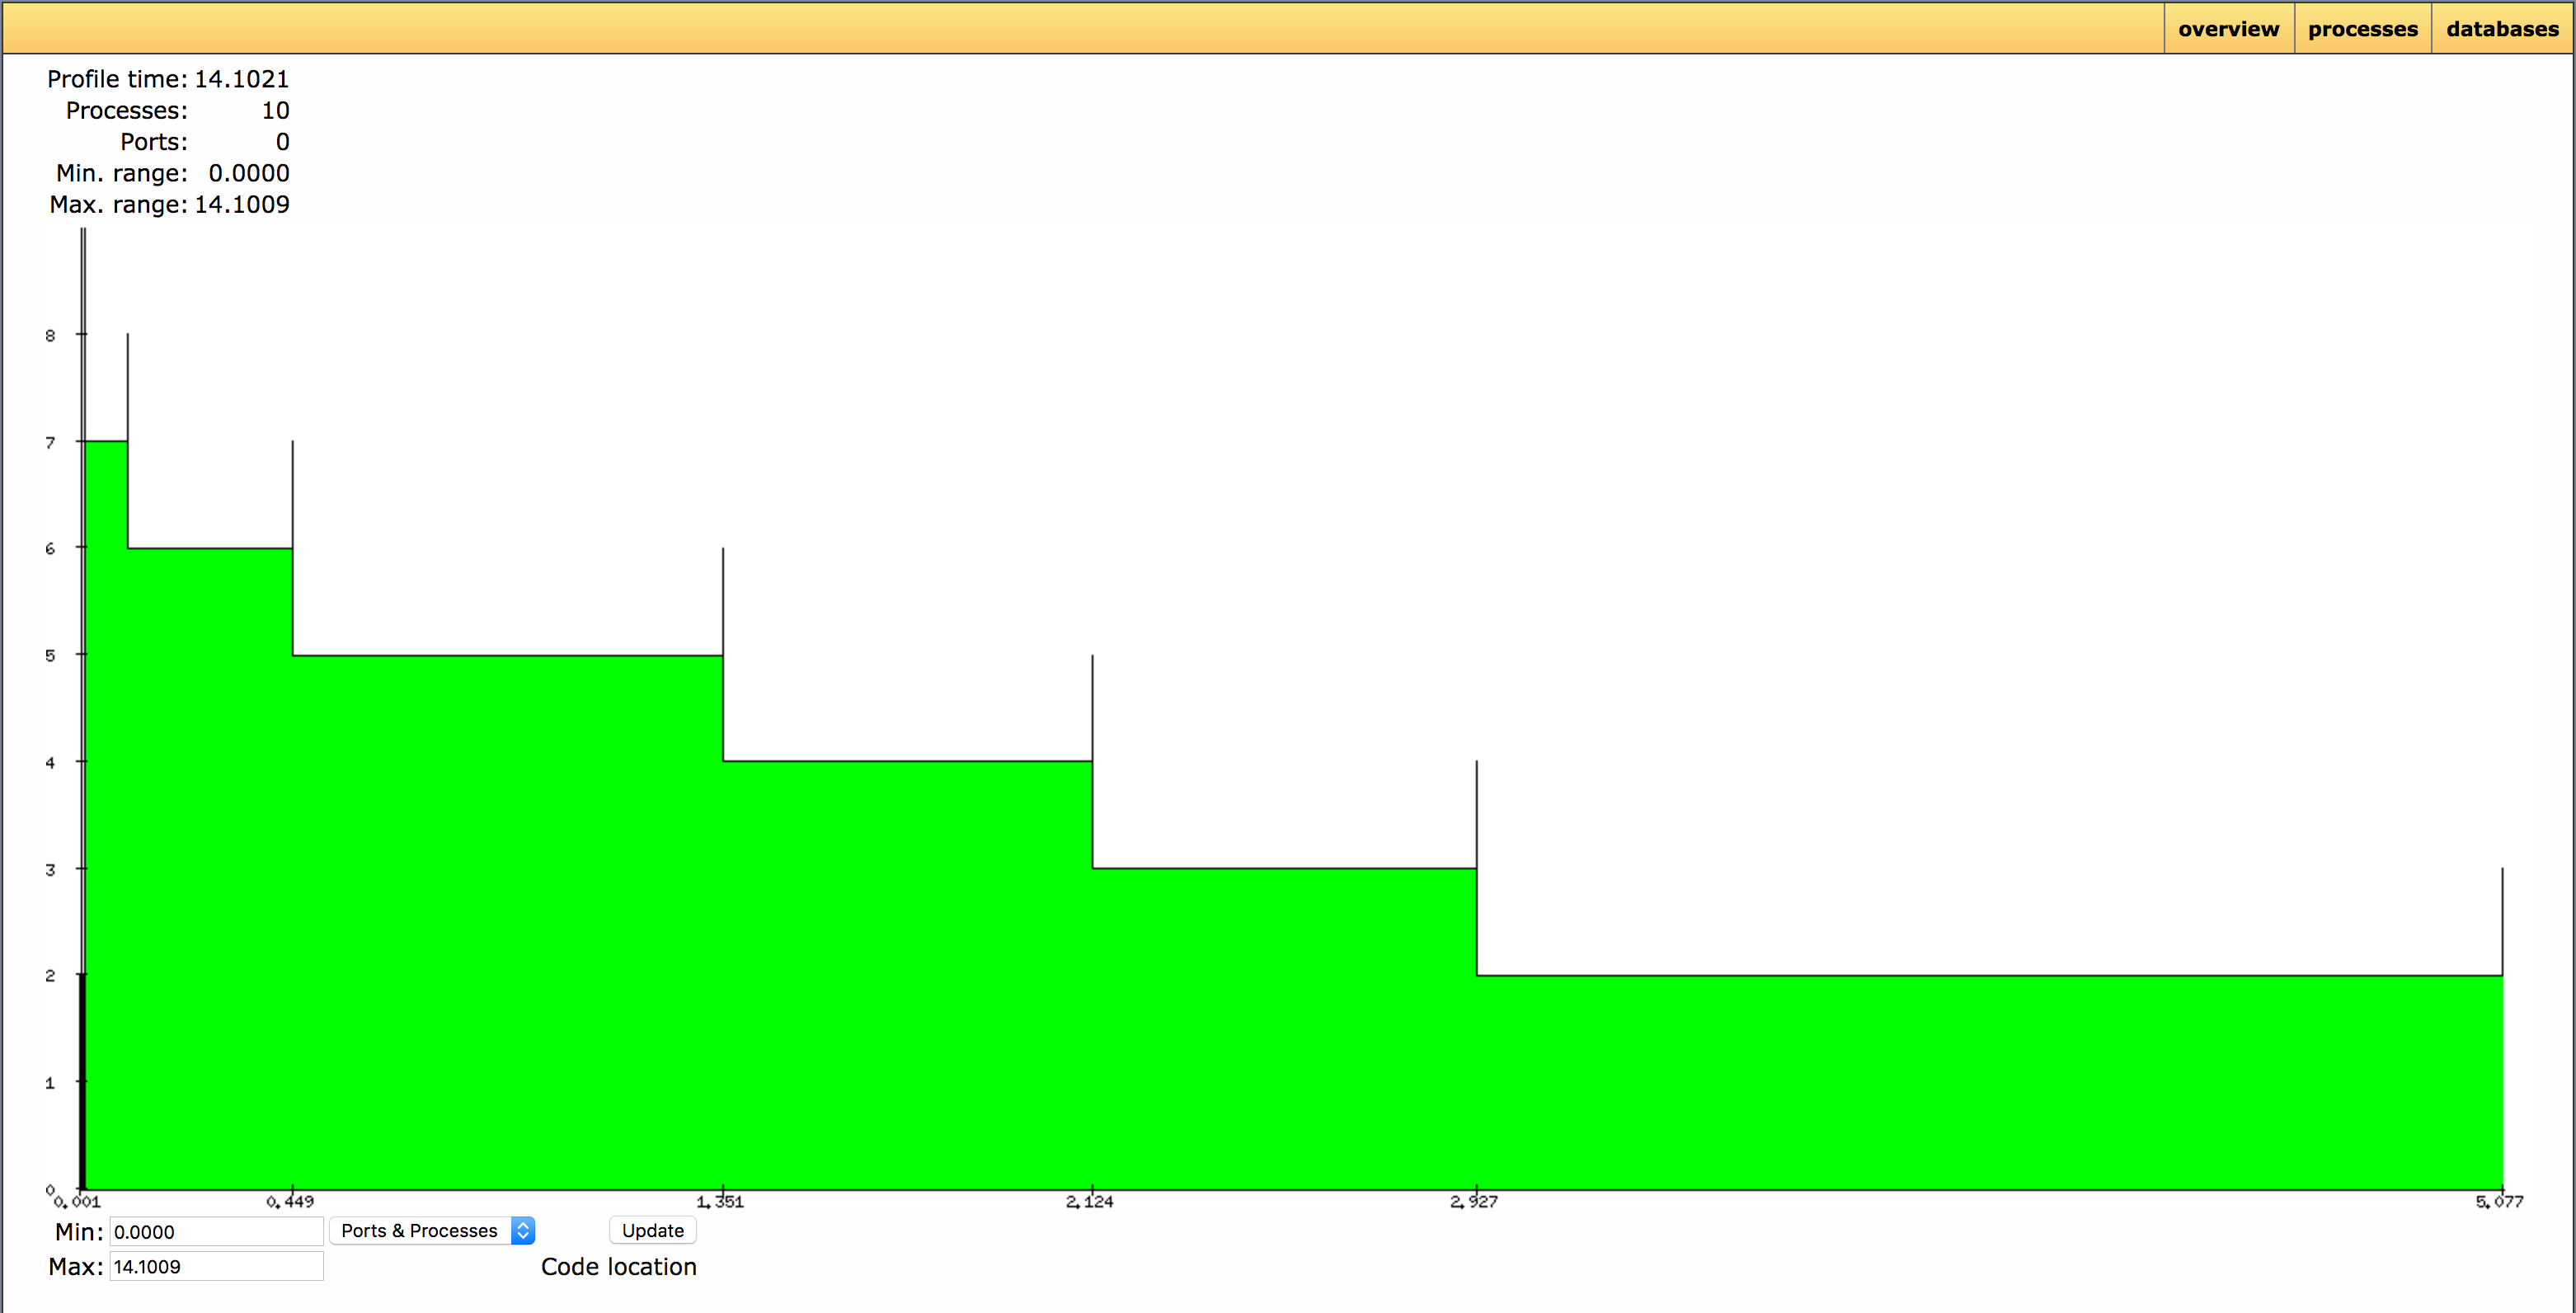
\includegraphics[scale=0.2]{bencmarks_in_parallel}
\caption{The percept graph showing the parallelism we obtain when running benchmarks in parallel.}
\label{fig:benchpar}
\end{center}
\end{figure}

The speedup of the total running time is $1.37$. As expected, the solving of every single puzzle takes more time than benchmark but the total running time for solving all puzzles is faster since puzzles are solved in parallel. Having one dedicated core for each puzzle would probably give the same running time as benchmark for each single puzzle, resulting in a total solving time equal to the solving time of the hardest individual puzzle.

\newpage
%%%%%%%%%%%%%%%%%%%%%%
\section{Parallelizing the solver}
As suggested in the lab PM, we tried two different approaches for parallelizing the solver. Both solutions are described below.

%%%%%%%
\subsection{Refine in parallel}
Our modified code for running solve in parallel can be found in the file \textit{labBGroup11\textunderscore pRefine.erl}.

Refining rows in parallel seems like a bad idea, because refining a row is a small task relative to the cost of parallelizing. Looking at figure \ref{fig:refparzoom} we can see that most of the time there is only 1 process working. At least, we were not able to build any solution using this approach that did not give a huge slowdown compared to benchmark. Below is the output of our submitted solution. Because of the long running time, the output is from a run with only one execution per puzzle instead of a hundred.

\begin{lstlisting}[escapeinside={(*}{*)}, tabsize=2]
{14422518,
[{wildcat,1.471},
 {diabolical,158.002},
 {vegard_hanssen,792.523},
 {challenge,93.865},
 {challenge1,11270.986},
 {extreme,429.075},
 {seventeen,1676.574}]}
\end{lstlisting}

\begin{figure}[!htb]
\begin{center}
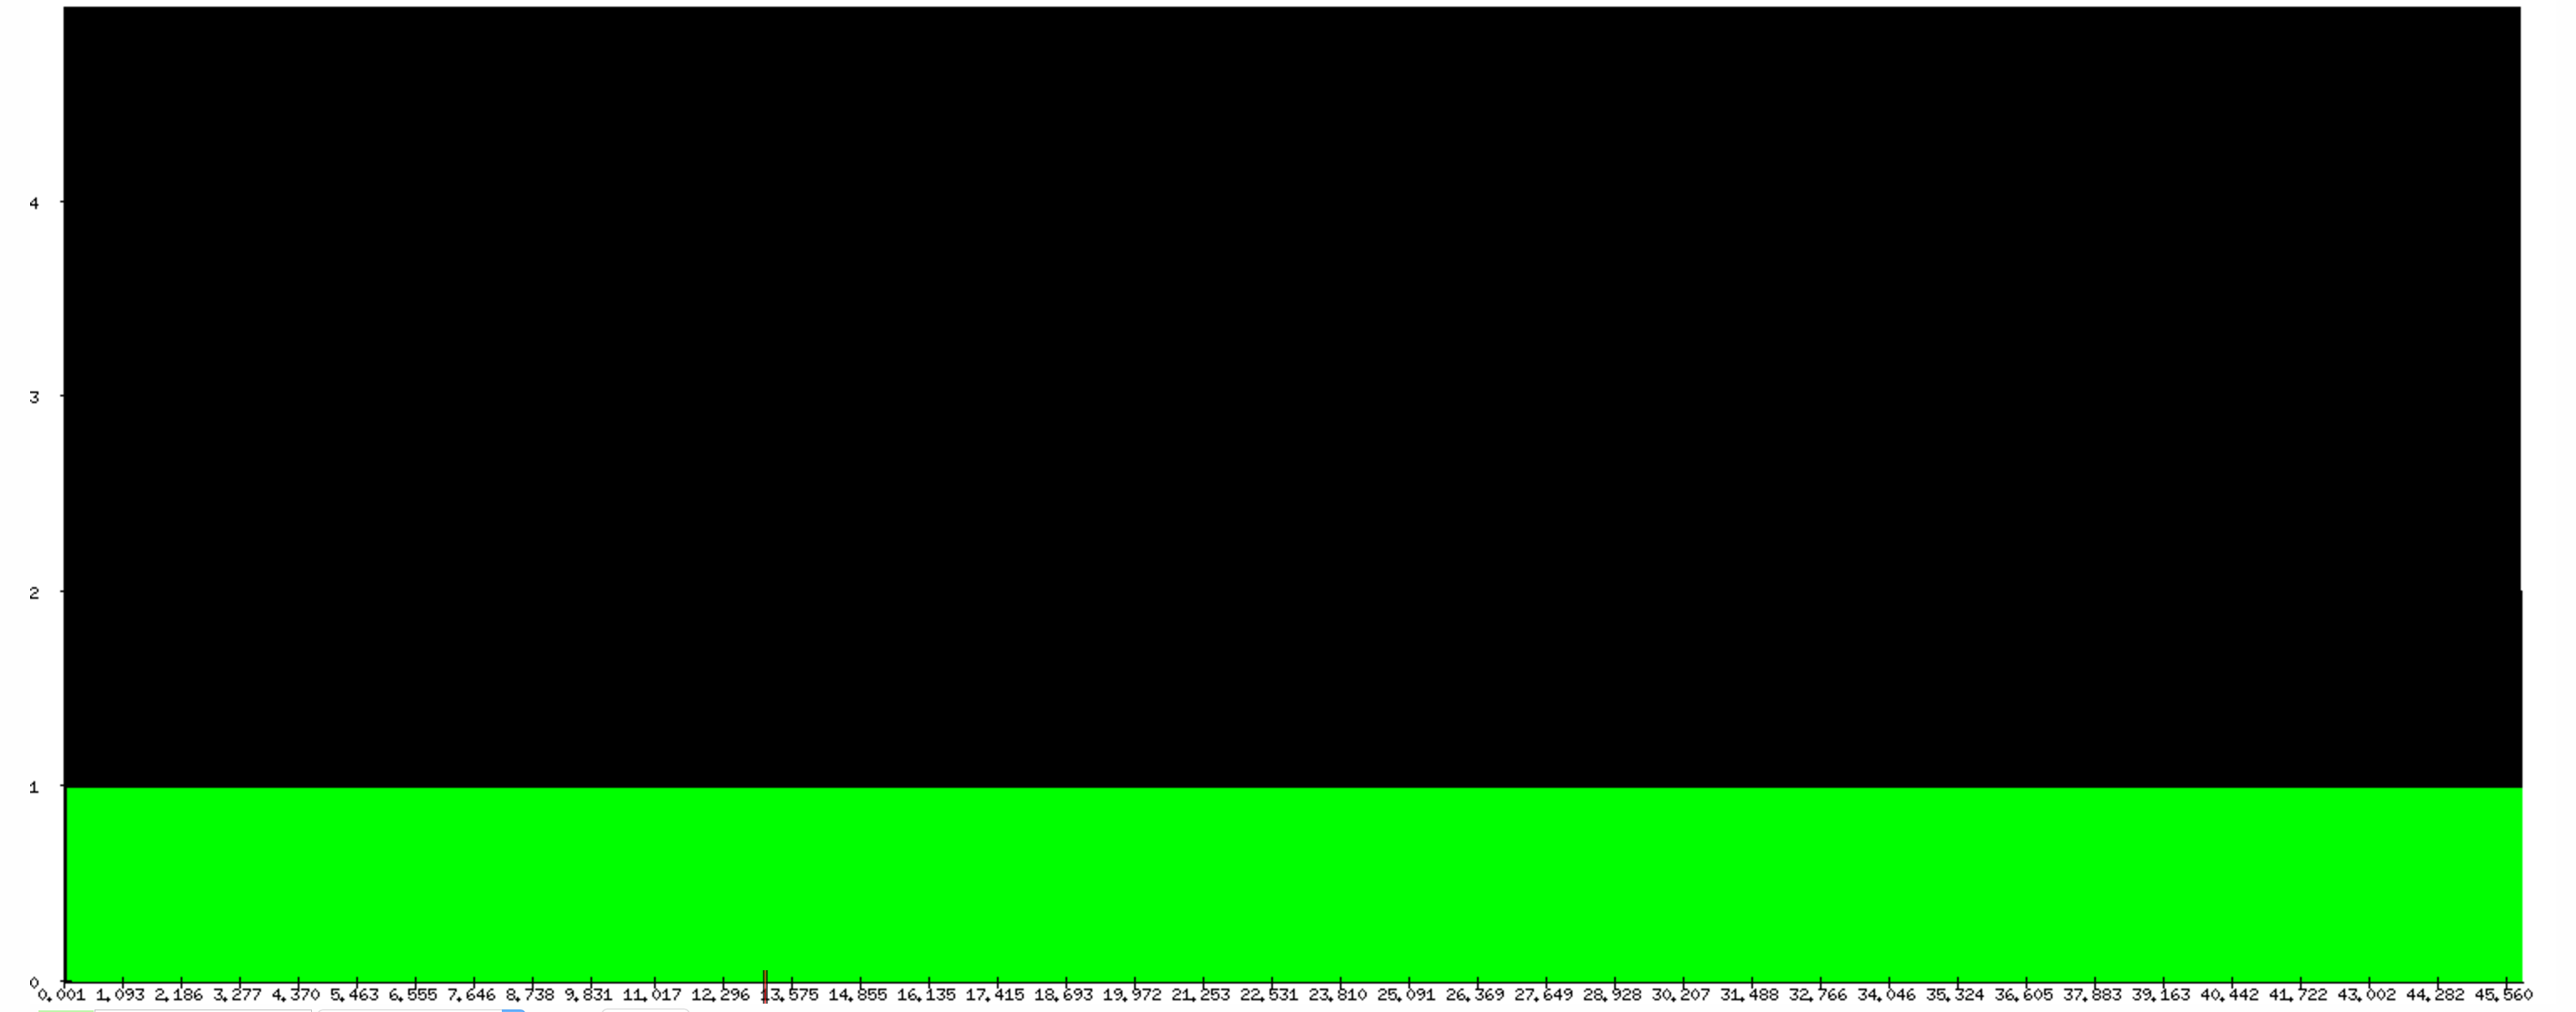
\includegraphics[scale=0.2]{refine_in_parallel}
\caption{The percept graph showing the parallelism we obtain when refining rows in parallel.}
\label{fig:refpar}
\end{center}
\end{figure}
\begin{figure}[!htb]
\begin{center}
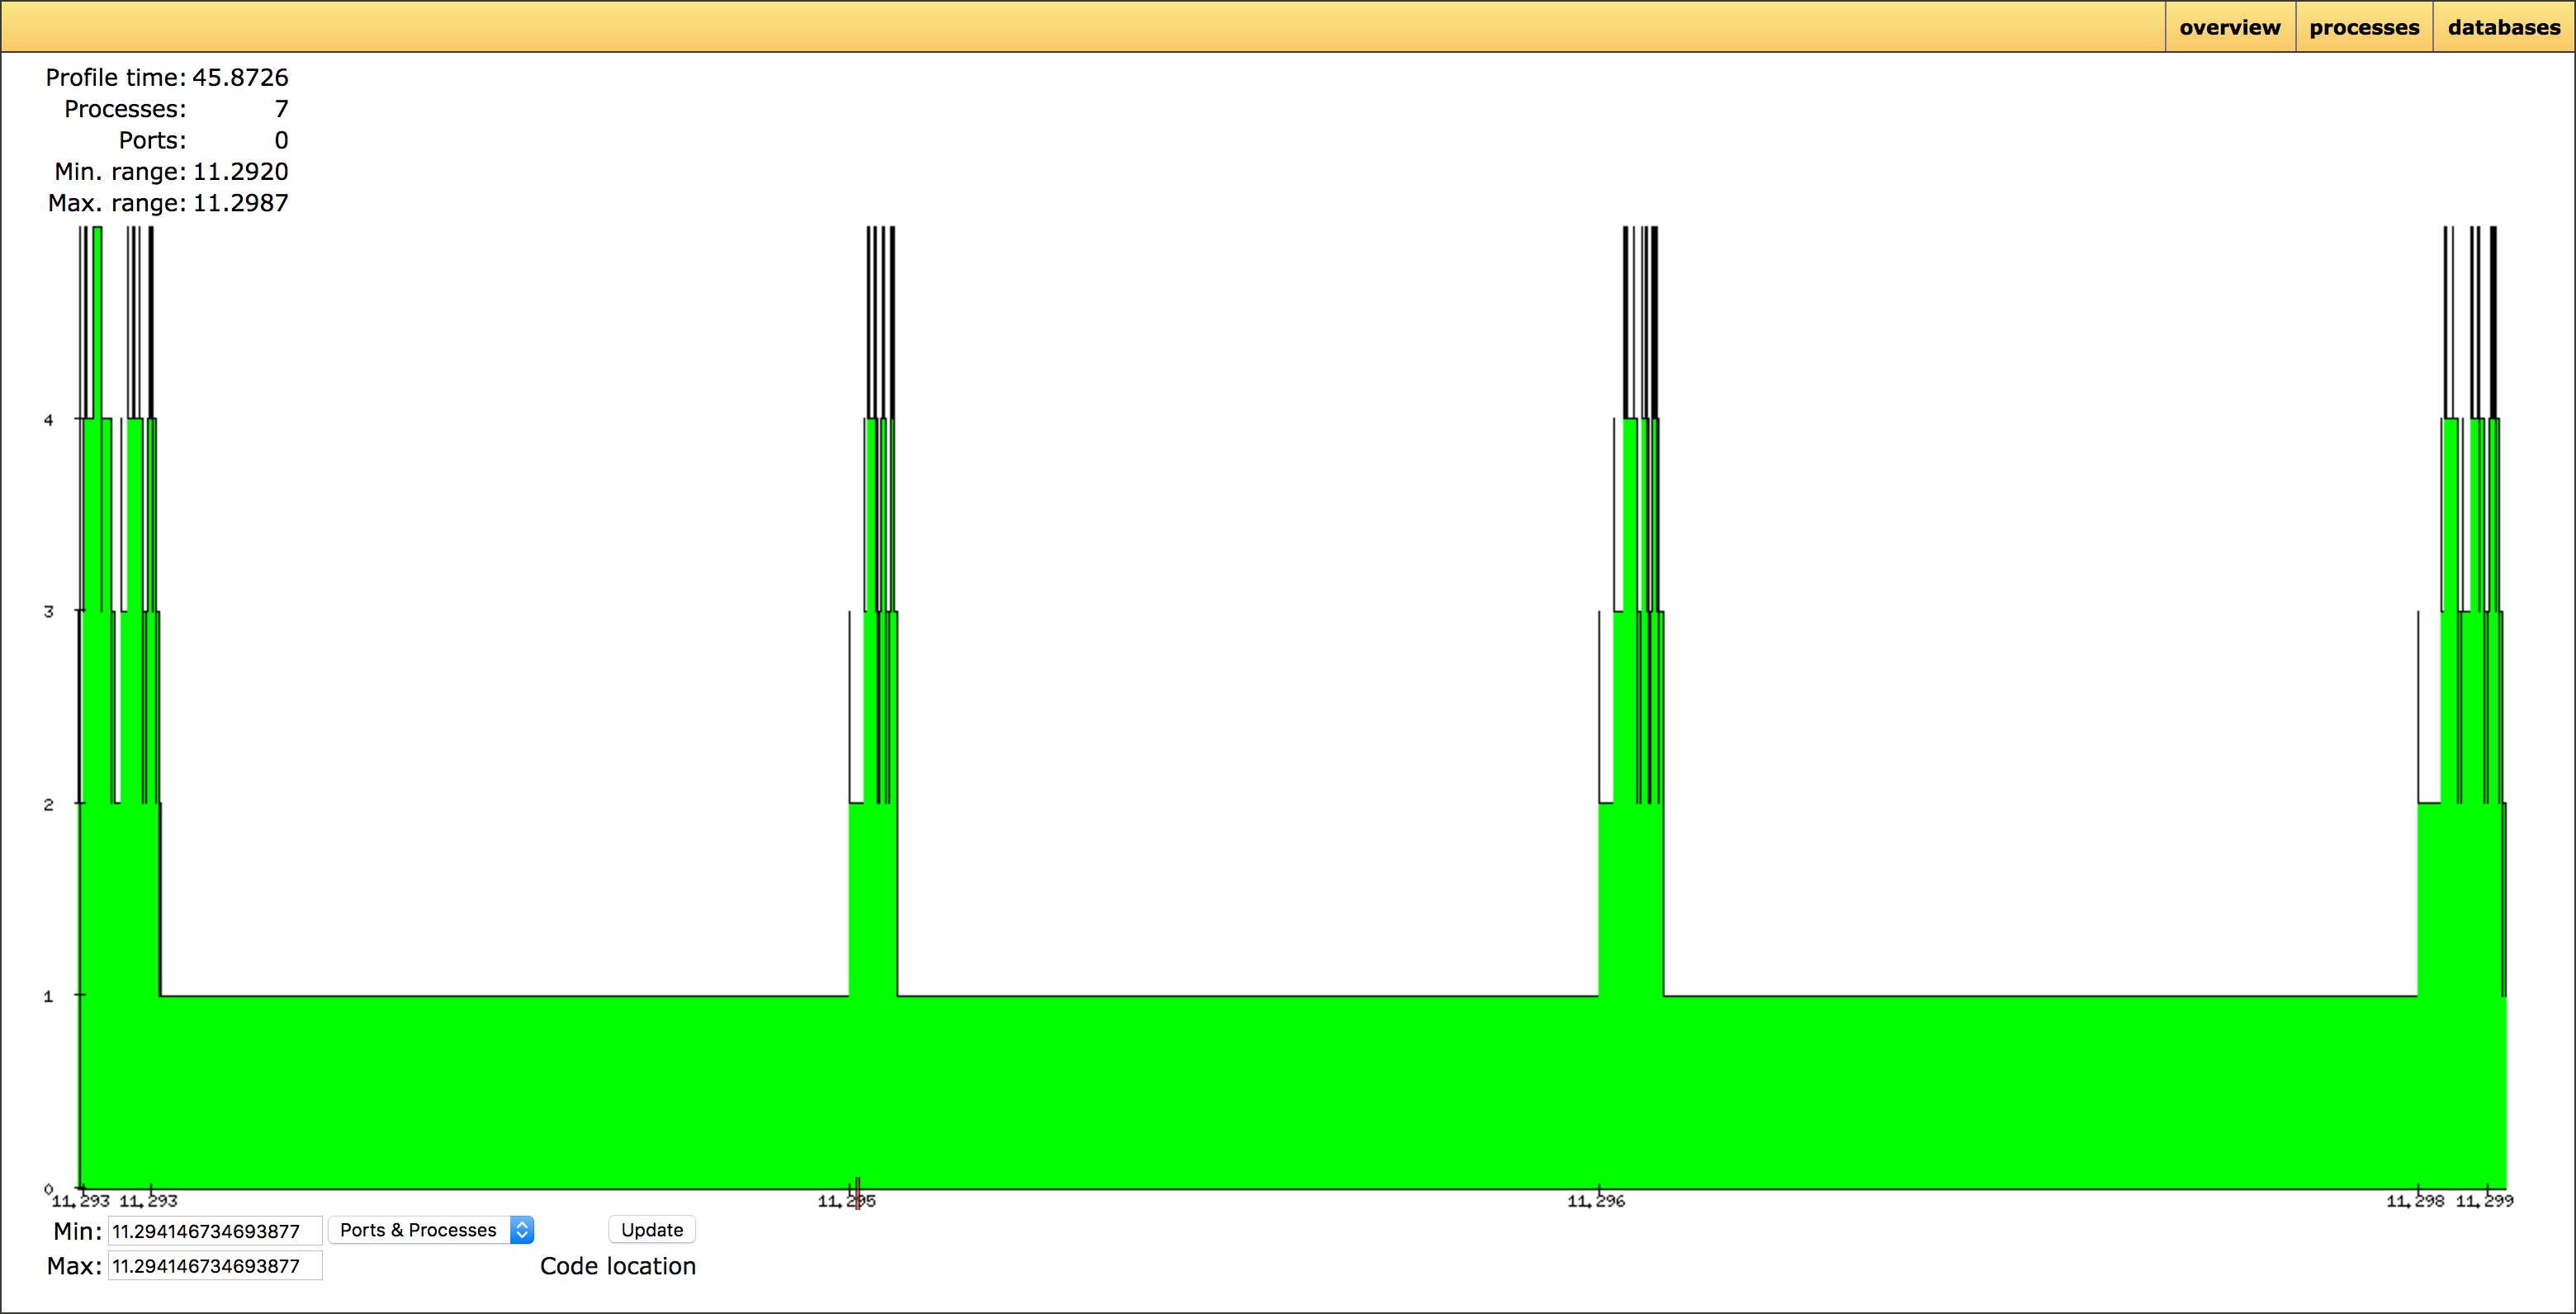
\includegraphics[scale=0.2]{refine_in_parallel_zoom}
\caption{A zoom of the percept graph showing the parallelism we obtain when refining rows in parallel.}
\label{fig:refparzoom}
\end{center}
\end{figure}

If running time scales linearly, a run with $100$ executions per puzzle would take $24$ minutes, which is a slowdown with a factor $22.61$.

%%%%%%%
\subsection{Solve in parallel}
Our modified code for running solve in parallel can be found in the file \textit{labBGroup11\textunderscore pSolve.erl}.

We use a pool of workers working in parallel. When a worker needs to guess a value and has more work to do, it asks another worker to do the next task and continues recursively with the rest of the tasks. If no other worker is available, it does the task by itself.

The output when running this code is the following:
\begin{lstlisting}[escapeinside={(*}{*)}, tabsize=2]
{31195465,
[{wildcat,0.45045999999999997},
 {diabolical,5.8761},
 {vegard_hanssen,33.04286},
 {challenge,3.36858},
 {challenge1,238.24194},
 {extreme,10.85971},
 {seventeen,20.114849999999997}]}
\end{lstlisting}

\begin{figure}[!htb]
\begin{center}
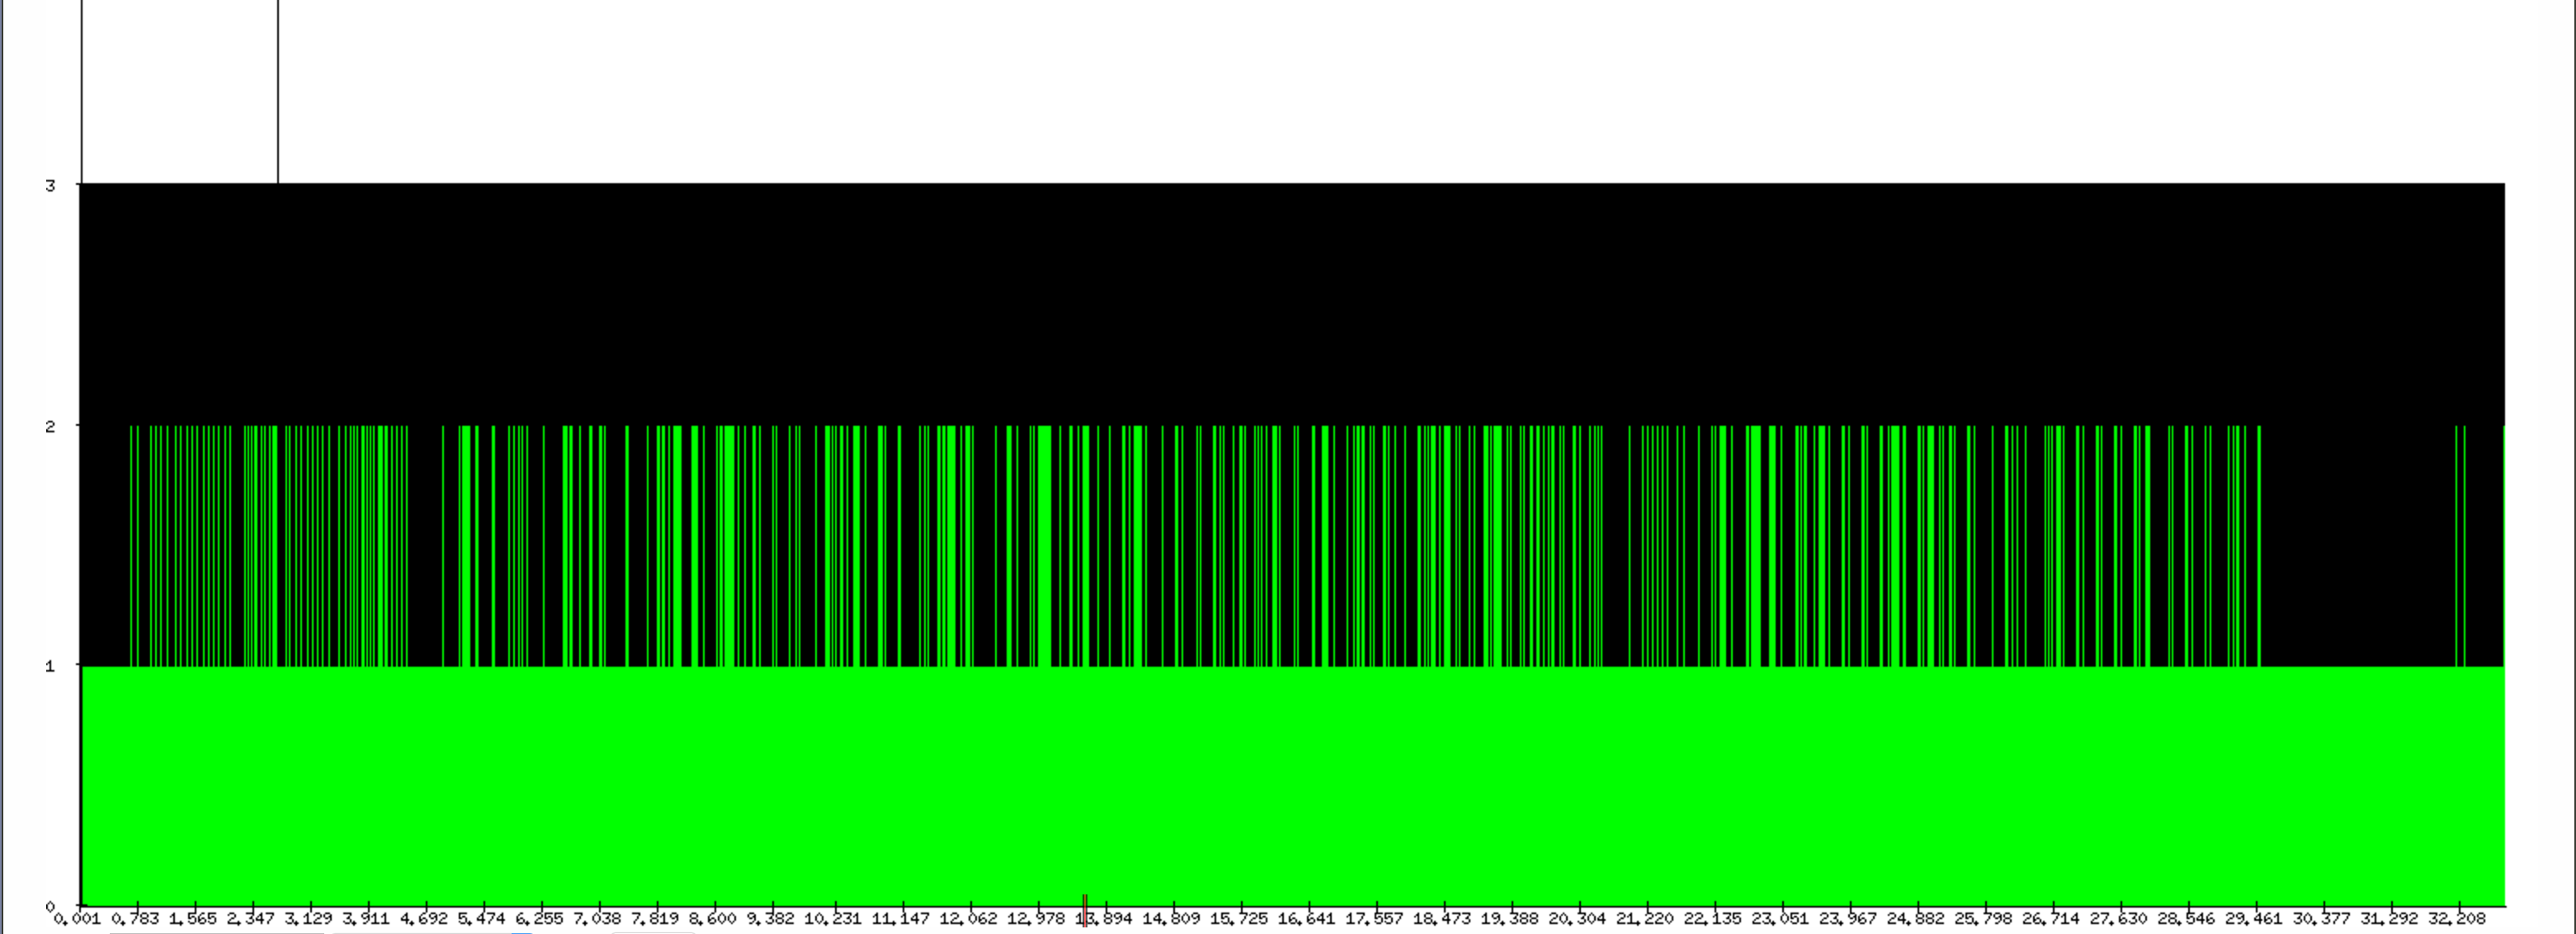
\includegraphics[scale=0.2]{Speculative_2_workers}
\caption{The percept graph showing the parallelism we obtain when running solve in parallel.}
\label{fig:solpar}
\end{center}
\end{figure}
\begin{figure}[!htb]
\begin{center}
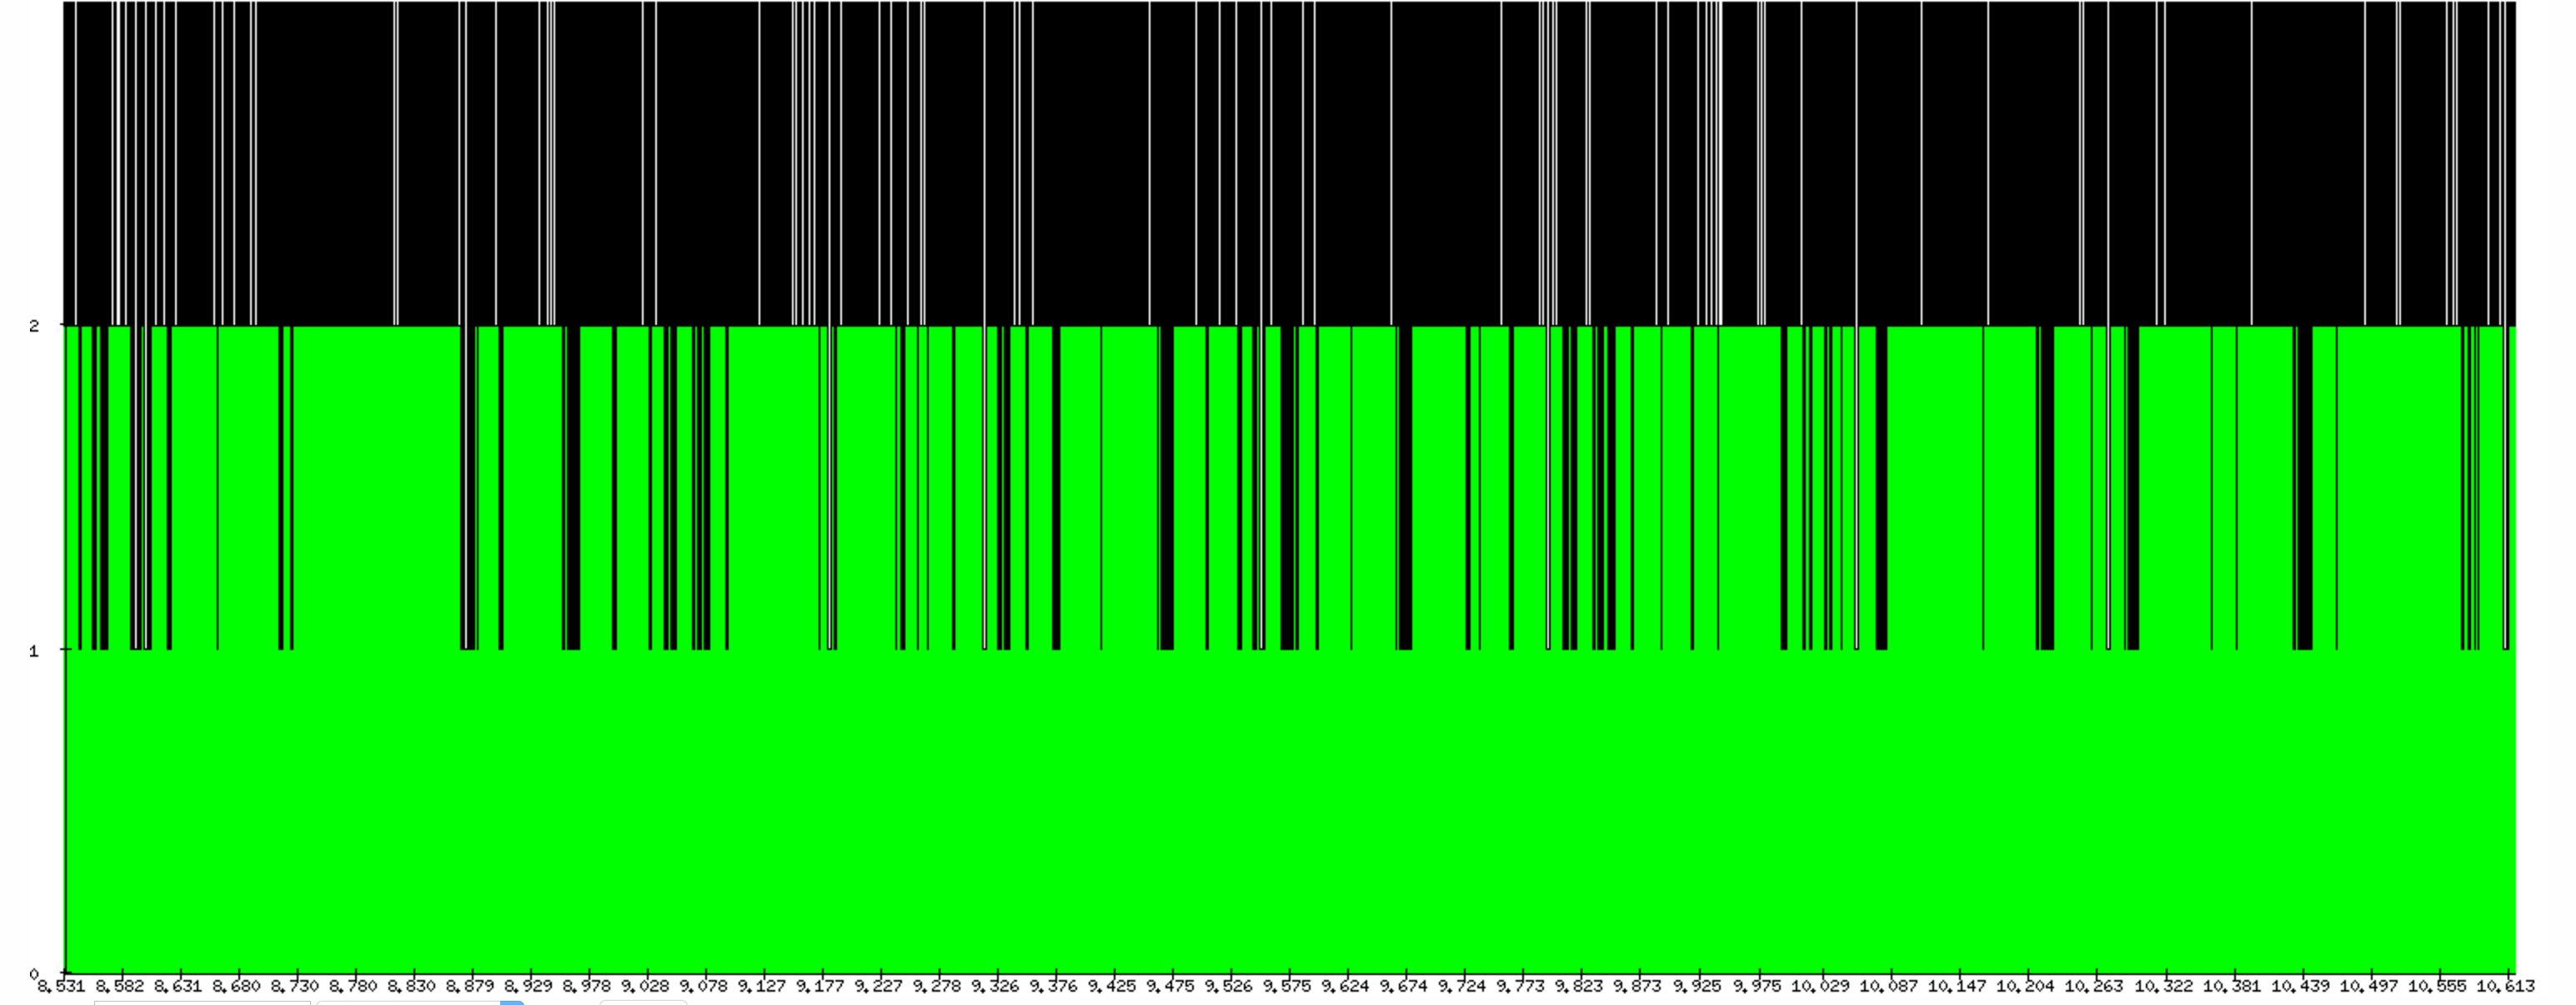
\includegraphics[scale=0.2]{Speculative_2_workers_zoom}
\caption{A zoom of the percept graph showing the parallelism we obtain when running solve in parallel.}
\label{fig:solparzoom}
\end{center}
\end{figure}

The speedup of the total running time is $2.04$.

Since this is our best speedup, we compute the speedups for every single puzzle:\\
wildcat: $1.03$\\
diabolical: $8.95$\\
vegard\textunderscore hanssen: $3.56$\\
challenge: $2.33$\\
challenge1: $1.72$\\
extreme: $0.96$\\
seventeen: $1.90$\\
\textbf{Geometric mean: $2.19$}

For a machine with only two cores, this seems like a really good result. We observe that we got very different speedups for different puzzles. This is expected since there is an element of "luck" affecting the running time for a specific instance of a depth first search like this one, depending on which branch you start exploring relative to where the solution is located.

\end{document}
